\documentclass{beamer} 
\usepackage[utf8]{inputenc}
\usepackage[T1]{fontenc} 
\usepackage[slovene]{babel} 
\usepackage{lmodern}
\usepackage{amsfonts} 
\usepackage{enumitem} 
\usepackage{mathtools}
\usepackage{amsmath}
\usepackage{amsthm} 

\newcommand{\overbar}[1]{\mkern 1.5mu\overline{\mkern-1.5mu#1\mkern-1.5mu}\mkern 1.5mu}


\usetheme{Warsaw}
\beamertemplatenavigationsymbolsempty
\setbeamertemplate{caption}[numbered]

\title{Schwarzov princip zrcaljenja za harmonične funkcije}
\author{Matej Novoselec}
\institute[UL FMF]{FMF Fakulteta za matematiko in fiziko}
\date{5. december 2022}


\theoremstyle{definition}
\newtheorem{defi}{Definicija}[section]
\theoremstyle{definition}
\newtheorem{op}[defi]{Opomba}
\newtheorem{trditev}{Trditev}
\newtheorem{lema}{Lema}
\newtheorem{izrek}{Izrek}

\begin{document}
%----------------------------------
\begin{frame}
   \titlepage
\end{frame}
%----------------------------------
%---------------------------------
\begin{frame}{Harmonične funkcije}
   \begin{block}{Definicija}
    Funkcija $u(x_1, x_2, \dots, x_n)$ je harmonična, če velja
    $$
    \frac{\partial^2 u}{\partial x_1 ^ 2} +  \frac{\partial^2 u}{\partial x_2 ^ 2} + \dots + \frac{\partial^2 u}{\partial x_n ^ 2} = 0.
    $$
    Operatorju $\Delta  = \frac{\partial^2}{\partial x_1 ^ 2} +  \frac{\partial^2}{\partial x_2 ^ 2} + \dots + \frac{\partial^2}{\partial x_n ^ 2}$ pravimo Laplaceov operator in pišemo
    $$
    \Delta u = 0.
    $$
   \end{block}
   \pause
   Harmonične funkcije lahko gledamo kot realne dele holomorfnih funkcij.
\end{frame}
\begin{frame}{Princip maksima}
   \begin{alertblock}{Izrek (Princip maksima za holomorfne funkcije)}
      Naj bo $D \subseteq \mathbb{C}$ območje v $\mathbb{C}$ in $f: D \rightarrow \mathbb{C}$ holomorfna in omejena funkcija.
      Tedaj je $f$ konstantna ali pa lokalnega maksimuma na $D$ ne zavzame.      
      \newline
      \pause 
      Če je $f$ definirana in zvezna na $\overbar{D}$, potem maksimum zavzame na $\partial D$.
   \end{alertblock}
   \pause
   \begin{exampleblock}{Princip maksima za harmonične funkcije}
      Dovolj je zahtevati, da je $f$ na $D$ harmonična in omejena, ter na $\overbar{D}$ zvezna. 
   \end{exampleblock}
\end{frame}
%----------------------------------
\begin{frame}{Dirichletov problem za enotski disk}
   \begin{alertblock}{Problem (Dirichletov problem za enotski disk)}
      Podano imamo zvezno funkcijo $h$ na $\partial \mathbb{D}$. 
      Radi bi skonstruirali harmonično funkcijo $\widetilde{h}$ na $\mathbb{D}$, tako da ko $z \in \mathbb{D} \to \xi \in \partial \mathbb{D} $, tudi $\widetilde{h}(z) \to h(\xi)$.
      \newline
      \pause
      Iščemo funkcijo, zvezno na $\overline{\mathbb{D}}$ in harmonično na $\mathbb{D}$, tako da se bo njena zožitev na $\partial \mathbb{D}$ ujemala s $h$.
   \end{alertblock}
   \begin{exampleblock}{Poskusimo rešiti...}
   \pause
   Če razširitev obstaja je enolično določena.
   \pause
   \newline
   Zapišimo $h = h(e^{i \theta})$ in poskusimo na enostavnih funkcijah $h$.
   \end{exampleblock}
\end{frame}

\begin{frame}{Poissonovo jedro}
   \begin{block}{Definicija}
      \textbf{Poissonovo jedro} je funkcija definirana s predpisom
      $$
         P_r(\theta) = \sum_{k = -\infty}^{\infty}{r^{|k|} e^{i k \theta}}\text{, kjer je}~\theta \in [-\pi, \pi]~\text{in}~ r < 1.
      $$
   \end{block}
   \pause
   \begin{alertblock}{Spomnimo se...}
      Naj $D$ zadošča pogojem za Greenovo formulo. 
      Naj bo $f \in \mathcal{O}(D) \cap \mathcal{C}^1(\overline{D})$. 
      Za $z \in D$ velja Cauchyjeva formula: 
      $$
      f(z) = \frac{1}{2 \pi i} \int_{\partial D}{\frac{f(\xi)}{\xi - z}~d\xi}.
      $$
      \pause
      \newline
      Funkciji 
      $
      (\xi, z) \mapsto \frac{1}{\xi - z}
      $
      pravimo Cauchyjevo jedro.

   \end{alertblock}
\end{frame}

\begin{frame}{Poissonov integral}
   Poskusimo sedaj iz druge smeri \dots

   \begin{block}{Definicija}
      \textbf{Poissonov integral}, ki ga označimo z~$\widetilde{h}(z)$, od $h(e^{i\theta})$ je funkcija na enotskem disku s predpisom
      $$
      \widetilde{h}(z) = \int_{-\pi}^{\pi}{h(e^{i\phi}) P_r(\theta - \phi)~\frac{d\phi}{2 \pi}}~\text{, kjer}~~z = r e^{i\theta} \in \mathbb{D}.
      $$
   \end{block}
   \pause
   \begin{exampleblock}{Izrek (Poissonov integral)}
      Naj bo $h(e^{i \theta})$ zvezna funkcija na enotski krožnici. 
      Potem nam zgoraj definiran Poissonov integral $\widetilde{h}(z)$ ponuja razširitev funckije $h$ do zvezne funckije na $\overline{\mathbb{D}}$, harmonične v $\mathbb{D}$ in velja, da
      se njena zožitev na $\partial \mathbb{D}$ ujema s $h$.
   \end{exampleblock}
\end{frame}

\begin{frame}{Lastnost povprečne vrednosti}
   \begin{block}{Definicija} 
      Zvezna funckija $h(z)$ ima na območju $D$ lastnost povprečne vrednosti, če za vsak $z_0$ iz $D$ velja, 
      da je $h(z_0)$ povprečje vrednosti $h(z)$, kjer $z$ teče po majhni krožnici s središčem v $z_0$.
   \end{block}
   \pause
   Holomorfne funkcije imajo lastnost povprečne vrednosti. 
   \pause
   \begin{exampleblock}{Izrek (Karakterizacija harmoničnih funkcij)}
      Naj bo $h(z)$ zvezna funkcija na območju $D$. 
      Potem je $h(z)$ harmonična na D natanko tedaj, ko ima $h(z)$ lastnost povprečne vrednosti na $D$.
   \end{exampleblock}
\end{frame}

\begin{frame}
   \begin{alertblock}{Spomnimo se...}
      \textbf{Izrek (Morera):} \newline
      Naj bo $f: D \to \mathbb{C}$ zvezna in $D$ odprta. 
      Denimo, da za vsak zaprt trikotnik $T \subseteq D$ velja 
      $$
      \int_{\partial T} {f(\xi)~d\xi} = 0
      $$
      Tedaj je $f$ holomorfna na $D$.
   \end{alertblock}
\end{frame}

\begin{frame}
   \begin{exampleblock}{Izrek (Schwarzov princip zrcaljenja za harmonične funckije)}
      Naj bo $D \subseteq \mathbb{C}$ območje simetrično glede na realno os. 
      Označimo $D^{+} = D \cap \{\text{Im} > 0\}$. 
      Naj bo $u(z): D^{+} \to \mathbb{R}$ harmonična funkcija, za katero velja, da gre $u(z) \to 0$, ko gre $z \in D^{+}$ proti poljubni točki $D \cap \mathbb{R}$. 
      \newline
      Potem obstaja harmonična razširitev $u(z)$ na $D$, ki je eksplicitno podana s predpisom $u(\bar{z}) = - u(z)$ za $z \in D$.
   \end{exampleblock}
   \pause
   %\begin{figure}
   %\begin{center}
   %   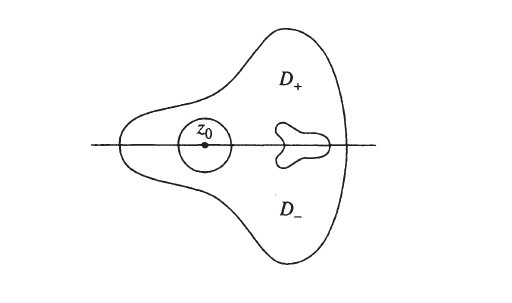
\includegraphics[width=0.70\textwidth]{schwarzov_princip_zrcaljenja.png}
   %\end{center}
   %\end{figure}
\end{frame}

% -------------------------------------------------------------------
%---------------------------------------------------------
\end{document}
